% Grundlegende Dokumenteneigenschaften gemäß DHBW-Vorgaben
\documentclass[a4paper,fontsize=11pt,oneside,parskip=half,headings=normal]{scrreprt} 
\usepackage{amsmath}
\usepackage{caption}
\usepackage{braket}


% \usepackage[
%             colorlinks=false,
%             citebordercolor={1 1 1},
%             filebordercolor={1 1 1},
%             linkbordercolor={1 1 1},
%             menubordercolor={1 1 1},
%             pagebordercolor={1 1 1},
%             urlbordercolor={1 1 1},
%             runbordercolor={1 1 1},
%             pagebackref=false,
%             plainpages=false,
%             % pdfpagelabels,
%             % ngerman
%             ]{hyperref}



\newcommand{\code}[1]{\texttt{#1}}
% \usepackage{showframe} % nur für Kontrolle der Ränder 

%%% Präambel einbinden (mit Festlegungen gemäß DHBW-Vorgaben) %%%
%%% Präambel %%%
% hier sollten keine Änderungen erforderlich sein
%
\usepackage[utf8]{inputenc}   % Zeichencodierung UTF-8 für Eingabe-Dateien
\usepackage[T1]{fontenc}      % Darstellung von Umlauten im PDF

\usepackage{ifthen}

\usepackage{listings}         % für Einbindung von Code-Listings
\lstset{numbers=left,numberstyle=\tiny,numbersep=5pt,texcl=true}
\lstset{literate=             % erlaubt Sonderzeichen in Code-Listings 
  {Ö}{{\"O}}1
{Ä}{{\"A}}1
{Ü}{{\"U}}1
{ß}{{\ss}}2
{ü}{{\"u}}1
{ä}{{\"a}}1
{ö}{{\"o}}1
{€}{{\euro}}1
}

\usepackage[
  inner=35mm,outer=15mm,top=25mm,
  bottom=20mm,foot=12mm,includefoot
]{geometry}                 % Einstellungen für Ränder

\usepackage[ngerman]{babel} % Spracheinstellungen Deutsch
\usepackage[babel,german=quotes]{csquotes} % deutsche Anf.zeichen
\usepackage{enumerate}      % anpassbare Nummerier./Aufz.
\usepackage{graphicx}       % Einbinden von Grafiken
\usepackage[onehalfspacing]{setspace} % anderthalbzeilig

\usepackage{blindtext}      % Textgenerierung für Testzwecke
\usepackage{color}          % Verwendung von Farbe 

\usepackage{acronym}        % für ein Abkürzungsverzeichnis

\usepackage[                % Biblatex
  backend=biber,
  bibstyle=lib/template/_dhbw_authoryear,maxbibnames=99,
  citestyle=authoryear,
  uniquename=true, useprefix=true,
  bibencoding=utf8]{biblatex}
%kein Punkt am Ende bei \footcite
%http://www.golatex.de/footcite-ohne-punkt-am-schluss-t4865.html
\renewcommand{\bibfootnotewrapper}[1]{\bibsentence#1}


%Reihenfolge der Autorennamen
%   
% http://golatex.de/viewtopic,p,80448.html#80448
% Argumente: siehe http://texwelt.de/blog/modifizieren-eines-biblatex-stils/
\DeclareNameFormat{sortname}{% Bibliographie
  \ifnum\value{uniquename}=0 % Normalfall
    \ifuseprefix%
      {%
         \usebibmacro{name:family-given}
           {\namepartfamily}
           {\namepartgiveni}
           {\namepartprefix}
           {\namepartsuffixi}%
       }
      {%
         \usebibmacro{name:family-given}
           {\namepartfamily}
           {\namepartgiveni}
           {\namepartprefixi}
           {\namepartsuffixi}%
       }%
  \fi
  \ifnum\value{uniquename}=1% falls nicht eindeutig, abgek. Vorname 
      {%
         \usebibmacro{name:family-given}
           {\namepartfamily}
           {\namepartgiveni}
           {\namepartprefix}
           {\namepartsuffix}%
       }%
  \fi
  \ifnum\value{uniquename}=2% falls nicht eindeutig, ganzer Vorname 
      {%
         \usebibmacro{name:family-given}
           {\namepartfamily}
           {\namepartgiven}
           {\namepartprefix}
           {\namepartsuffix}%
       }%
  \fi   
  \usebibmacro{name:andothers}}

\DeclareNameFormat{labelname}{% für Zitate
  \ifnum\value{uniquename}=0 % Normalfall
    \ifuseprefix%
      {%
         \usebibmacro{name:family-given}
           {\namepartfamily}
           {\empty}
           {\namepartprefix}
           {\namepartsuffixi}%
       }
      {%
         \usebibmacro{name:family-given}
           {\namepartfamily}
           {\empty}
           {\namepartprefixi}
           {\namepartsuffixi}%
       }%
  \fi
  \ifnum\value{uniquename}=1% falls nicht eindeutig, abgek. Vorname 
      {%
         \usebibmacro{name:family-given}
           {\namepartfamily}
           {\namepartgiveni}
           {\namepartprefix}
           {\namepartsuffix}%
       }%
  \fi
  \ifnum\value{uniquename}=2% falls nicht eindeutig, ganzer Vorname 
      {%
         \usebibmacro{name:family-given}
           {\namepartfamily}
           {\namepartgiven}
           {\namepartprefix}
           {\namepartsuffix}%
       }%
  \fi   
  \usebibmacro{name:andothers}}
      
  
\DeclareFieldFormat{extrayear}{% = the 'a' in 'Jones 1995a'
  \iffieldnums{labelyear}
    {\mknumalph{#1}}
    {\mknumalph{#1}}}        

\renewcommand*{\multinamedelim}{\addslash}
\renewcommand*{\finalnamedelim}{\addslash}
\renewcommand*{\multilistdelim}{\addslash}
\renewcommand*{\finallistdelim}{\addslash}

\renewcommand{\nameyeardelim}{~}

% Literaturverzeichnis: Doppelpunkt zwischen Name (Jahr): Rest 
% http://de.comp.text.tex.narkive.com/Tn1HUIXB/biblatex-authoryear-und-doppelpunkt
\renewcommand{\labelnamepunct}{\addcolon\addspace}

% damit die Darstellung für Vollzitate von Primärquellen in 
% Fußnoten später auf "nicht fett" geändert werden kann 
% (nur für Zitate von Sekundärliteratur relevant)
\newcommand{\textfett}[1]{\textbf{#1}}

% für Zitate von Sekundärliteratur:
\newcommand{\footcitePrimaerSekundaer}[4]{%
  \renewcommand{\textfett}[1]{##1}%
  \footnote{\fullcite[#2]{#1}, zitiert nach \cite[#4]{#3}}%  
  \renewcommand{\textfett}[1]{\textbf{##1}}%
}

% Im Literaturverzeichnis: Autor (Jahr) fett
\renewbibmacro*{author}{%
  \ifboolexpr{%
    test \ifuseauthor%
    and
    not test {\ifnameundef{author}}
  }
    {\usebibmacro{bbx:dashcheck}
       {\bibnamedash}
       {\usebibmacro{bbx:savehash}%
        \textfett{\printnames{author}}%
        \iffieldundef{authortype}
          {\setunit{\addspace}}
          {\setunit{\addcomma\space}}}%
     \iffieldundef{authortype}
       {}
       {\usebibmacro{authorstrg}%
        \setunit{\addspace}}}%
    {\global\undef\bbx@lasthash
     \usebibmacro{labeltitle}%
     \setunit*{\addspace}}%
  \textfett{\usebibmacro{date+extrayear}}}

% Sonderfall: Quelle ohne Autor, aber mit Herausgeber
% Name des Herausgebers wird fett gedruckt
\renewbibmacro*{bbx:editor}[1]{%
  \ifboolexpr{%
    test \ifuseeditor%
    and
    not test {\ifnameundef{editor}}
  }
    {\usebibmacro{bbx:dashcheck}
       {\bibnamedash}
       {\textfett{\printnames{editor}}%
        \setunit{\addcomma\space}%
        \usebibmacro{bbx:savehash}}%
     \usebibmacro{#1}%
     \clearname{editor}%
     \setunit{\addspace}}%
    {\global\undef\bbx@lasthash
     \usebibmacro{labeltitle}%
     \setunit*{\addspace}}%
  \textfett{\usebibmacro{date+extrayear}}}

% Anpassungen für deutsche Sprache
\DefineBibliographyStrings{ngerman}{%
	nodate = {{o.J.}},
	urlseen = {{Abruf:}},
	ibidem = {{ebenda}}
}

% keine Anführungszeichen beim Titel im Literaturverzeichnis
\DeclareFieldFormat[article,book,inbook,inproceedings,manual,misc,phdthesis,thesis,online,report]{title}{#1\isdot}

\newcommand{\literaturverzeichnis}{%
% nur Literaturverzeichnis
% (als eigenes Kapitel)
\phantomsection% 
\addcontentsline{toc}{chapter}{Literaturverzeichnis}
\spezialkopfzeile{Literaturverzeichnis}
\defbibheading{lit}{\chapter*{Literaturverzeichnis}}% 
\label{chapter:quellen}
\printbibliography[heading=lit,notkeyword=ausblenden]
} % mit DHBW-spezifischen Einstellungen

\usepackage{hyperref}       % URL-Formatierung, klickbare Verweise

\usepackage{tocloft}        % für Verzeichnis der Anhänge

\newcounter{anhcnt}
\setcounter{anhcnt}{0}
\newlistof{anhang}{app}{}

\newcommand{\anhang}[1]{%
  \refstepcounter{anhcnt}
  \setcounter{anhteilcnt}{0}
  \section*{Anhang \theanhcnt: #1}
  \addcontentsline{app}{section}{\protect\numberline{Anhang \theanhcnt}#1}\par
}

\newcounter{anhteilcnt}
\setcounter{anhteilcnt}{0}

\newcommand{\anhangteil}[1]{%
  \refstepcounter{anhteilcnt}
  \subsection*{Anhang~\arabic{anhcnt}/\arabic{anhteilcnt}: #1}
  \addcontentsline{app}{subsection}{\protect\numberline{Anhang \theanhcnt/\arabic{anhteilcnt}}#1}\par
}

\renewcommand{\theanhteilcnt}{Anhang \theanhcnt/\arabic{anhteilcnt}}

% vgl. S. 4 Paket-Beschreibung tocloft 	
% Einrückungen für Anhangverzeichnis
\makeatletter
\newcommand{\abstaendeanhangverzeichnis}{
  \renewcommand*{\l@section}{\@dottedtocline{1}{0em}{5.5em}}
  \renewcommand*{\l@subsection}{\@dottedtocline{2}{2.3em}{6.5em}}
}
\makeatother

% Abbildungs- und Tabellenverzeichnis
% Bezeichnungen
\renewcaptionname{ngerman}{\figurename}{Abb.}
\renewcaptionname{ngerman}{\tablename}{Tab.}
% Einrückungen
\makeatletter
\renewcommand*{\l@figure}{\@dottedtocline{1}{0em}{2.3em}}
\renewcommand*{\l@table}{\@dottedtocline{1}{0em}{2.3em}}
\makeatother


\usepackage{chngcntr}                % fortlaufende Zähler für Fußnoten, Abbildungen und Tabellen
\counterwithout{figure}{chapter}
\counterwithout{table}{chapter}
\counterwithout{footnote}{chapter}

\usepackage[automark]{scrlayer-scrpage}
%% Definitionen für Kopf- und Fußzeile auf normalen Seiten
\defpagestyle{kopfzeile}
{% Kopfdefinition
  (\textwidth,0pt)    % Länge der oberen Linie,Dicke der oberen Linie       
  {} % Definition für linke Seiten im doppelseitigen Layout
  {} % Definition für rechte Seiten im doppelseitigen Layout      
  {  % Definition für Seiten im einseitigen Layout
	\makebox[0pt][l]{\rightmark}% 
	\makebox[\linewidth]{}% 
  }        
  (\textwidth, 0.4pt) % Untere Linienlänge, Untere Liniendicke
}
{% Fußdefinition
  (\textwidth,0pt)    % Obere Linienlänge, Obere Liniendicke
  {} % Definition für linke Seiten im doppelseitigen Layout
  {} % Definition für rechte Seiten im doppelseitigen Layout
  {  % Definition für Seiten im einseitigen Layout
    \makebox[\linewidth]{}%
    \makebox[0pt][r]{\pagemark}%
  }
  (\textwidth, 0pt)   % Länge der unteren Linie,Dicke der unteren Linie
}

%% Definitionen für Kopf- und Fußzeile auf ersten Seiten eines Kapitels
\defpagestyle{kapitelkopfzeile}
{% Kopfdefinition
  (\textwidth,0pt)    % Länge der oberen Linie,Dicke der oberen Linie       
  {} % Definition für linke Seiten im doppelseitigen Layout
  {} % Definition für rechte Seiten im doppelseitigen Layout      
  {}  % Definition für Seiten im einseitigen Layout
  (\textwidth, 0pt) % Untere Linienlänge, Untere Liniendicke
}
{% Fußdefinition
  (\textwidth,0pt)    % Obere Linienlänge, Obere Liniendicke
  {} % Definition für linke Seiten im doppelseitigen Layout
  {} % Definition für rechte Seiten im doppelseitigen Layout
  {  % Definition für Seiten im einseitigen Layout
    \makebox[\linewidth]{}%
    \makebox[0pt][r]{\pagemark}%
  }
  (\textwidth, 0pt)   % Länge der unteren Linie,Dicke der unteren Linie
}

%% Definitionen für Kopf- und Fußzeile im Anhang und bei Quellenverzeichnisse
\newcommand{\spezialkopfzeileBezeichnung}{}
\defpagestyle{spezialkopfzeile}
{% Kopfdefinition
  (\textwidth,0pt)    % Länge der oberen Linie,Dicke der oberen Linie       
  {} % Definition für linke Seiten im doppelseitigen Layout
  {} % Definition für rechte Seiten im doppelseitigen Layout      
  {  % Definition für Seiten im einseitigen Layout
	\makebox[0pt][l]{\spezialkopfzeileBezeichnung}% 
	\makebox[\linewidth]{}% 
  }        
  (\textwidth, 0.4pt) % Untere Linienlänge, Untere Liniendicke
}
{% Fußdefinition
  (\textwidth,0pt)    % Obere Linienlänge, Obere Liniendicke
  {} % Definition für linke Seiten im doppelseitigen Layout
  {} % Definition für rechte Seiten im doppelseitigen Layout
  {  % Definition für Seiten im einseitigen Layout
    \makebox[\linewidth]{}%
    \makebox[0pt][r]{\pagemark}%
  }
  (\textwidth, 0pt)   % Länge der unteren Linie,Dicke der unteren Linie
}
            
\newcommand\spezialkopfzeile[1]{%
  \renewcommand\spezialkopfzeileBezeichnung{#1}
  \pagestyle{spezialkopfzeile}
}
                
% Standard-Pagestyle auswählen
\pagestyle{kopfzeile}

% keine Kopfzeile anzeigen auf Seiten, auf denen ein 
% Kapitel beginnt oder das Inhalts-/Abbildungs-/Tabellenverzeichnis steht 
\renewcommand{\chapterpagestyle}{kapitelkopfzeile}
\tocloftpagestyle{kapitelkopfzeile}

		 % für schöne Kopfzeilen 

\usepackage{textcomp}            % erlaubt EUR-Zeichen in Eingabedatei
\usepackage{eurosym}             % offizielles EUR-Symbol in Ausgabe
\renewcommand{\texteuro}{\euro}  % ACHTUNG: nach hyperref aufrufen!

\usepackage{scrhack}             % stellt Kompatibilität zw. KOMA-Script
% (scrreprt) und anderen Paketen her

% Anpassung der Abstände bei Kapitelüberschriften
% (betrifft auch Inhalts-, Abbildungs- und Tabellenverzeichnis)
\renewcommand*\chapterheadstartvskip{\vspace*{-\topskip}}
\newcommand{\myBeforeTitleSkip}{1mm}
\newcommand{\myAfterTitleSkip}{10mm}
\setlength\cftbeforetoctitleskip{\myBeforeTitleSkip}
\setlength\cftbeforeloftitleskip{\myBeforeTitleSkip}
\setlength\cftbeforelottitleskip{\myBeforeTitleSkip}

\setlength\cftaftertoctitleskip{\myAfterTitleSkip}
\setlength\cftafterloftitleskip{\myAfterTitleSkip}
\setlength\cftafterlottitleskip{\myAfterTitleSkip}
%%% Ende der Präambel %%%


%% Einlesen der Konfigurationdatei
% Typ der Arbeit (für Deckblatt und ehrenwörtliche Erklärung) - bitte Zutreffendes auswählen
% 1. Projektarbeit
% 2. Projektarbeit
% Seminararbeit
% Bachelorarbeit
\newcommand{\bootstrapPaperType}{2. Projektarbeit}

% Thema der Arbeit (für ehrenwörtliche Erklärung, ohne Umbrüche)
\newcommand{\bootstrapPaperTitle}{tbd.}

% Ggf. Untertitel der Arbeit (falls dies nicht benötigt wird, das zweite Klammerpaar leer lassen, nicht das Kommando löschen!)
\newcommand{\bootstrapPaperSubtitle}{}

% Vorname, Name der Autorin/des Autors (für Titelseite und Metadaten)
\newcommand{\bootstrapAuthor}{Jonas Michel}

% Abgabedatum (\today wird durch das Datum zum Zeitpunkt der Kompilation ersetzt/Datum kann auch manuell in die Klammern geschrieben werden)
% Beispiel: 10. Mai 2021
\newcommand{\bootstrapDueDate}{20.11.2023}

% Fakultät der Arbeit festlegen
\newcommand{\bootstrapFaculty}{Wirtschaft und Gesundheit}

% Studiengang festlegen.
\newcommand{\bootstrapMajor}{Wirtschaftsinformatik}

% Kurs festlegen
\newcommand{\bootstrapCourseID}{WWI2021F} % Kursnummer (Beispiel: WWI2018F)

% Informationen bezüglich des dualen Partners (Arbeitsgeber/Firma)
\newcommand{\bootstrapCompanyAdvisorGender}{m} % m/f/x für die verschiedenen Geschlechter
\newcommand{\bootstrapCompanyName}{IBM} % Name der Firma
\newcommand{\bootstrapCompanyAdvisorDetails}{Dr.~Stefan Kister} % Name und Titel der betreuenden Person in der Firma.
\newcommand{\bootstrapCompanyAdvisorPosition}{Quantum Ambassador} % Funktion der betreuenden Person in der Firma (Job Titel).

% Informationen bzgl. der wissenschaftliche Betreuung
\newcommand{\bootstrapUniversityAdvisorDetails}{Prof.~Dr.~Kai Holzweißig} % Name und Titel der Person der wiss. Betreuung.
\newcommand{\bootstrapUniversityAdvisorPosition}{Studiengangsleiter WWI2021F} % Funktion der Person der wiss. Betreuung.


%%% Name der eigenen Literatur-Datenbank %%%
\bibliography{lib/pa_2.bib}

\begin{document}
%%% Deckblatt einbinden %%% 
% Support command for generating the gender conform advisor term.
\newcommand{\genderedAdvisor}[1]{
        \ifthenelse{\equal{#1}{m}}
        {Betreuer}
        {\ifthenelse{\equal{#1}{f}}{Betreuerin}{Betreuungsperson}}
}

% Support command to generate the gender conform advisor term including an article.
\newcommand{\genderedAdvisorArticle}[1]{
        \ifthenelse{\equal{#1}{m}}
        {des Betreuers}
        {\ifthenelse{\equal{#1}{f}}{der Betreuerin}{der Betreuungsperson}}
}

\thispagestyle{empty}

\begin{spacing}{1}
        \begin{center}
                ~\vspace{0mm}

                % Titel der Arbeit
                {\sffamily
                        \LARGE
                        \textbf{\bootstrapPaperTitle}

                        \bigskip
                        \textbf{\bootstrapPaperSubtitle}
                }

                \vspace{15mm}

                % Typ der Arbeit
                {\Large \bootstrapPaperType}

                \vspace{1cm}

                % Datum festlegen
                vorgelegt am \bootstrapDueDate

                \vspace{15mm}

                % Fakultät festlegen
                Fakultät \bootstrapFaculty
                \medskip

                % Studiengang festlegen
                Studiengang \bootstrapMajor
                \medskip

                % Kurs festlegen
                Kurs \bootstrapCourseID

                \vspace{10mm}

                von

                \vspace{10mm}

                % Autor/in/en/innen festlegen
                {\large\textsc{\bootstrapAuthor}}

                \vspace{10mm}
        \end{center}

        \vfill


        % HIER EDITIEREN: Name des Unternehmens, Name der Betreuerin/des Betreuers
        \begin{tabular}{ll}
                \genderedAdvisor{\bootstrapCompanyAdvisorGender}in der Ausbildungsstätte: & DHBW Stuttgart:                     \\
                \hspace{0.4\linewidth}                                                    &                                     \\
                \bootstrapCompanyName                                                     & \bootstrapUniversityAdvisorDetails  \\
                \bootstrapCompanyAdvisorDetails                                           & \bootstrapUniversityAdvisorPosition \\
                \bootstrapCompanyAdvisorPosition                                                                                \\
                \\
                Unterschrift\genderedAdvisorArticle{\bootstrapCompanyAdvisorGender}                                             \\
        \end{tabular}


        \vspace{1cm}
        %(etwas Platz für die Unterschrift der Betreuerin/des Betreuers aus der Ausbildungsstätte)
\end{spacing}

% falls ein Vertraulichkeitsvermerk erforderlich ist,
% die Kommentarzeichen in den nachfolgenden Zeilen entfernen:

%\begin{center}
%\small
%\textbf{Vertraulichkeitsvermerk}:
%Der Inhalt dieser Arbeit darf weder als Ganzes noch in Auszügen \\
%Personen außerhalb des Prüfungs- und Evaluationsverfahrens zugänglich gemacht werden, sofern keine anders lautende Genehmigung des Dualen Partners vorliegt. 
%\end{center}

% Meta-Daten für PDF-Datei basierend auf obigen Angaben
\hypersetup{pdftitle={\bootstrapPaperTitle}}
\hypersetup{pdfauthor={\bootstrapAuthor}}
\hypersetup{pdfsubject={\bootstrapPaperType\ DHBW Stuttgart \the\year}}


%%% Umstellung der Seiten-Nummerierung auf i, ii, iii ... %%%
\pagenumbering{Roman}

\begin{spacing}{1}

  %%% Inhaltsverzeichnis %%%
  \tableofcontents
  \clearpage

  %%% Abkürzungsverzeichnis %%%
  \chapter*{Abkürzungsverzeichnis}
\addcontentsline{toc}{chapter}{Abkürzungsverzeichnis}

\begin{acronym}[DHBW] 
    
% Argument definiert die Breite der ersten Spalte anhand des längsten vorkommenden Eintrags
\acro{LSTM}{Long Short Term Memory}
\acro{MAE}{Mean Absolute Error}
\acro{MSE}{Mean Squared Error}
\acro{QML}{Quantum Machine Learning}
\acro{QNN}{Quantum Neural Network}
\acro{QLSTM}{Quantum Long Short Term Memory}
\acro{RMSE}{Root Mean Squared Error}
\acro{RNN}{Recurrent Neural Network}
\acro{VQC}{Variational Quantum Circuit}

\end{acronym}
  \clearpage

  \thispagestyle{kapitelkopfzeile}

  %%% Abbildungsverzeichnis %%%
  \listoffigures
  \phantomsection

  %%% Einfügen des Abbildungsverzeichnisses in das Inhaltsverzeichnis %%%
  \addcontentsline{toc}{chapter}{Abbildungsverzeichnis}
  \clearpage

  %%% Tabellenverzeichnis %%%
  \listoftables
  \phantomsection

  %%% Einfügen des Tabellenverzeichnisses in das Inhaltsverzeichnis %%%
  \addcontentsline{toc}{chapter}{Tabellenverzeichnis}
  \cleardoublepage

\end{spacing}

%%% Umstellung der Seiten-Nummerierung auf 1, 2, 3 ... %%%
\pagenumbering{arabic}

%%% Beginn des eigentlichen Inhalts %%%
% Empfehlung: strukturieren Sie Ihren Text in einzelnen Dateien und binden Sie diese hier mit   \input{main_part/dateiname.tex} ein

\chapter{Einleitung}

Für die Verarbeitung von sequentiellen Daten, werden in der Praxis \ac{LSTM}-Modelle eingesetzt.\footcite[Vgl.][]{Sutskever2014} Beispielhaft hierfür sind die Anwendung bei Video zu Text Applikationen\footcite[Vgl.][]{Venugopalan2015} oder Timeseries Forecasting (Zeitreihenvorhersagung)\footcite[Vgl.][]{Chen2022}.
LSTM Architekturen sind außerdem die Basis der für GPT-3 benutzten Transformer Modelle.\footcite[Vgl.][S. 1ff.]{Vaswani2017}
In der aktuellen Literatur stellen \cite{Chen2022} und \cite{Yu2023} jeweils \ac{LSTM}-Architekturen vor, welche mit Quantum Computing erweitert wurden. Diese sogenannten \ac{QLSTM}-Architekturen, überzeugen mit einer höheren Genauigkeit und einer schnelleren Trainingszeit.
Währendessen gibt es immer mehr Unternehmen wie IBM\footcite[Vgl.][]{IBMQa}, Google\footcite[Vgl.][]{GoogleQa}, Microsoft\footcite[Vgl.][]{MicrosoftQ} und D-Wave\footcite[Vgl.][]{DWaveQ}, welche einsatzfähige Quantumcomputer entwickelt haben. Quantenfehlerverhinderung Algorithmen von IBM\footcite[Vgl.][]{Kim2023} und Google\footcite[Vgl.][]{Acharya2023} beschleunigen die Entwicklung zusätzlich.
Ein Quantumfortschritt lässt sich auch bei Machine Learning beobachten,~\cite{Abbas2021} zeigen, dass gewisse \ac{QNN}'s bessere Ergebnisse liefern und dazu schneller trainert werden können, als vergleichbare klassische Modelle.
In diversen physikalischen Experimenten haben \cite{Huang2021} einen aktueller Quantenvorteil im Vergleich zu klassischen Machine Learning Modellen nachgewiesen. 
Bei zyklischen wellenformigen Datensätzen, wie zum Beispiel einer Sinuskurve oder einem gedämpften Oszillator, haben spezielle \ac{QLSTM} Architekturen einen Vorteil gegenüber klassischen Modellen.\footcite[Vgl.][]{Chen2022}
Quantum Machine Learning Modelle eröffnen also perspektivisch die Aussicht, aktuelle hochkomplexe physikalische und chemische Probleme zu lösen.\footcite[Vgl.][S. 1]{Huang2021}

Wie gut ein \ac{QNN} performt hängt stark von der Architektur ab. Die Feature Map und der Variational Layer können beliebig angepasst werden und sind somit mäßgeblich für die Genauigkeit des Modells verantwortlich.\footcite[Vgl.][S. 404]{Abbas2021}
Wie sich verschiedene Feature Maps und Variational Layer auf unterschiedliche Datensätze auswirken ist hierbei noch zu untersuchen.\footcite[Vgl.][S. 407]{Abbas2021}
Aktuell gibt es einige wissenschaftliche Artikel\footcite[Vgl.][]{Chen2022,Yu2023,Qi2021} welche verschienden \ac{QLSTM} Architekturen benutzen um spezifische Datensätze zu bearbeiten. 
Diese Publikationen benutzten alle unterschidliche Feature Maps, Variational Layer und eigene Anwedungsfälle. Keine der Publikationen vergleicht die verschiedenen Architekturen miteinander oder wendet das Modell auf unterschiedliche Datensätze an.

Angesichts dieser beschriebenen Problematik stellt sich die Frage, \textbf{welche Art von \ac{QLSTM}-Architektur für unterschiedliche Datensätze am besten geeignet ist}. Das Ziel dieses Praxisarbeit besteht darin, vier verschiedene \ac{QLSTM}-Architekturen auf zwei unterschiedliche Datensätze anzuwenden, um sie im Anschluss miteinander zu vergleichen und zu evaluieren. 
Hierdurch soll ermittelt werden, ob eine spezifische \ac{QLSTM}-Architektur existiert, die für beide Datensätze als besonders geeignet ist, oder ob bestimmte Architekturen für spezifische Datensätze besser geeignet sind. 
Die Auswahl der Datensätze und Architekturen erfolgt dabei so, dass möglichst alle relevanten Aspekte dieser Fragestellung abgedeckt werden.

Forschungsmethode (Experiment) und Aufbau tbd.

\anhang{Literaturanalyse}

\anhangteil{Konzeptmatrix}\label{konzeptmatrix}
Um die gesamte Matrix übersichtlicher zu gestalten wurden die gängigen Abküzungen benutzt.
Quantum Data Encoding ist mit QDE abgekürzt, diese Abkürzung ist nicht im Abkürzungsverzeichnis zu finden, da sie nur für diese Tabelle benutzt wird.

Unter Artikel ist die bibtex ID des Artikels zu finden. Diese kann benutzt werden um den Artikel in der Literaturdatenbank zu finden.

\begin{tabular}{|c|c|c|c|c|c|}
    \hline
    \textbf{Artikel} & \multicolumn{5}{|c|}{\textbf{Konzepte}} \\
    \hline
     & \ac{LSTM} & \ac{QLSTM} & \ac{QML} & \ac{VQC} & QDE \\
    \hline
    xy & & & & & \\
    xy & & & & & \\
    xy & & & & & \\
    xy & & & & & \\
    xy & & & & & \\
    xy & & & & & \\
    xy & & & & & \\
    xy & & & & & \\
    xy & & & & & \\
    xy & & & & & \\
    xy & & & & & \\
    xy & & & & & \\
    xy & & & & & \\
    xy & & & & & \\
    xy & & & & & \\
    xy & & & & & \\
    xy & & & & & \\
    xy & & & & & \\
    xy & & & & & \\
    xy & & & & & \\
    xy & & & & & \\
    xy & & & & & \\
    xy & & & & & \\
    xy & & & & & \\
    xy & & & & & \\
    xy & & & & & \\
    xy & & & & & \\
    xy & & & & & \\
    xy & & & & & \\
    \hline
\end{tabular}

\begin{tabular}{|c|c|c|c|c|c|}
    \hline
    \textbf{Artikel} & \multicolumn{5}{|c|}{\textbf{Konzepte}} \\
    \hline
     & \ac{LSTM} & \ac{QLSTM} & \ac{QML} & \ac{VQC} & QDE \\
    \hline
    xy & & & & & \\
    xy & & & & & \\
    xy & & & & & \\
    xy & & & & & \\
    xy & & & & & \\
    xy & & & & & \\
    xy & & & & & \\
    xy & & & & & \\
    xy & & & & & \\
    xy & & & & & \\
    xy & & & & & \\
    xy & & & & & \\
    xy & & & & & \\
    xy & & & & & \\
    xy & & & & & \\
    xy & & & & & \\
    xy & & & & & \\
    xy & & & & & \\
    xy & & & & & \\
    xy & & & & & \\
    xy & & & & & \\
    xy & & & & & \\
    xy & & & & & \\
    xy & & & & & \\
    xy & & & & & \\
    xy & & & & & \\
    xy & & & & & \\
    xy & & & & & \\
    xy & & & & & \\
    xy & & & & & \\
    xy & & & & & \\
    xy & & & & & \\
    xy & & & & & \\
    xy & & & & & \\
    xy & & & & & \\
    xy & & & & & \\
    xy & & & & & \\
    xy & & & & & \\
    xy & & & & & \\
    \hline
\end{tabular}


\anhangteil{Suchbegriffe}\label{search}

\begin{tabular}{|c|c|c|c|c|c|c|}
    \hline
    \textbf{Suchbegriffe} & \multicolumn{6}{|c|}{\textbf{Konzepte}} \\
    \hline
     & \ac{LSTM} & \ac{QLSTM} & \ac{QML} & \ac{VQC} & QDE & Synonyme \\
    \hline
    xy & & & & & & \\
    xy & & & & & & \\
    xy & & & & & & \\
    xy & & & & & & \\
    xy & & & & & & \\
    xy & & & & & & \\
    xy & & & & & & \\
    \hline
\end{tabular}

\newpage


\chapter{Darlegen der Zielsetzung und Forschungsmethodik}

max. 2 Seiten

\section{Spezifizierung der Zielsetzung}
was wollen wir jetzt genau machen grober ausblick wie

\section{Forschungsmethodik}
wie funktioniert diese und warum wird sie benutzt? (Realtitsbsp)


\chapter{Design und Implementation des Experiments}\label{design}

bla bla bkla kommen wir nun zur implementierung und Entwicklung
hier wichitg aller code steht zur verfügung und kann gerunt werden. Alle benötigten schritte sind in der Arbeit vermekrt (umgebung und so weiter...)


\section{Entwicklungsumgebung}

Um die im folgenden Kapitel \ref{design} beschriebene Implementation lokal durchzuführen, ist es erforderlich, eine geeignete Entwicklungsumgebung aufzusetzen.
Die Programmierung erfolgte mithilfe von Visual Studio Code als Code-Editor. Die Python-Umgebung wurde unter Einsatz des Anaconda Navigators erstellt.
Der gesamte Quellcode basiert auf der Python Version 3.9.16.
Die wichtigsten Bibliotheken für eine erfolgreiche Implementation des nachfolgenden Artefaktes sind Qiskit und PyTorch.
Die Qiskit Version 0.43.0 ist notwendig, da in anderen Versionen von Qiskit Syntaxänderungen auftreten können.

Im Anhang \ref{conda} finden sich eine umfassende Aufstellung aller Abhängigkeiten und Bibliotheken, inklusive ihrer jeweiligen Versionsnummern, die während der Entwicklung und Ausführung des Artefakts zum Einsatz kamen. Zusätzlich sind dort detaillierte Informationen zur Entwicklungsumgebung sowie zur verwendeten Software verfügbar.




\section{Testdatensätze}

Zackige und runde Daten - erzeugt in: dort ausfürhlich dokuemntiert 
aber hier nochmal die websiten: 
Doku bei CODE!

\begin{figure}[htb]
    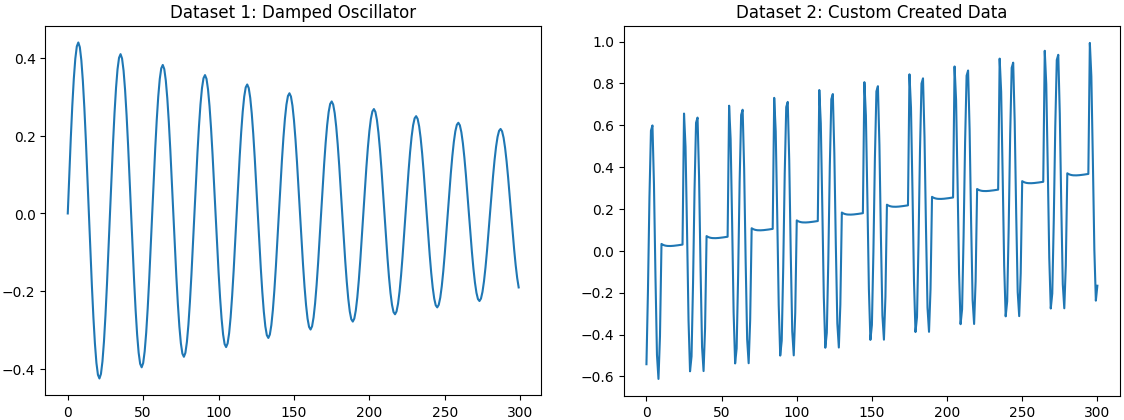
\includegraphics[width=16cm]{lib/graphics/data.png}
    \caption[Testdatensätze]{Testdatensätze}
    \label{abb:datasets}
\end{figure}



\section{Klassische LSTM Architektur Implementation}
als standard

\section{Quantum LSTM Architektur Implementation}
\subsection{Paper 1}
\subsection{Paper 2}

\section{Test Aufbau}

\section{Test Durchführung}


\chapter{Evaluation des Artefakts}

\section{Auswertung der Ergebnisse}

\section{Beantworten der Forschungsfrage}



\chapter{Kritische Reflextion}

2 Seiten pa

•  Zielsetzung der Arbeit kurz einführen


• Kritische Reflexion der Ergebnisse und
Methodik

• Implikationen der Arbeit für Theorie und Praxis

• Ausblick



%%% Ende des eigentlichen Inhalts %%%


%%% Beginn des Anhangs %%%
\chapter*{Anhang}
\addcontentsline{toc}{chapter}{Anhang}

\lstset{language=TeX,
    morekeywords={anhang, anhangteil}
}

% Definition des Anhangverzeichnis
\section*{Anhangverzeichnis}
\vspace{-8em}
\abstaendeanhangverzeichnis
\listofanhang
\clearpage

% Konfiguration der speziellen Kopfzeile für den Anhang
\spezialkopfzeile{Anhang}

% Hauptteil des Anhangs

% Mit \anhang{Abschnitt des Anhangs} fügt man ein Kapitel in dem Anhang hinzu z. B. Interview Transkripte

\anhang{Literaturanalyse}

\anhangteil{Konzeptmatrix}\label{konzeptmatrix}
Um die gesamte Matrix übersichtlicher zu gestalten wurden die gängigen Abküzungen benutzt.
Quantum Data Encoding ist mit QDE abgekürzt, diese Abkürzung ist nicht im Abkürzungsverzeichnis zu finden, da sie nur für diese Tabelle benutzt wird.

Unter Artikel ist die bibtex ID des Artikels zu finden. Diese kann benutzt werden um den Artikel in der Literaturdatenbank zu finden.

\begin{tabular}{|c|c|c|c|c|c|}
    \hline
    \textbf{Artikel} & \multicolumn{5}{|c|}{\textbf{Konzepte}} \\
    \hline
     & \ac{LSTM} & \ac{QLSTM} & \ac{QML} & \ac{VQC} & QDE \\
    \hline
    xy & & & & & \\
    xy & & & & & \\
    xy & & & & & \\
    xy & & & & & \\
    xy & & & & & \\
    xy & & & & & \\
    xy & & & & & \\
    xy & & & & & \\
    xy & & & & & \\
    xy & & & & & \\
    xy & & & & & \\
    xy & & & & & \\
    xy & & & & & \\
    xy & & & & & \\
    xy & & & & & \\
    xy & & & & & \\
    xy & & & & & \\
    xy & & & & & \\
    xy & & & & & \\
    xy & & & & & \\
    xy & & & & & \\
    xy & & & & & \\
    xy & & & & & \\
    xy & & & & & \\
    xy & & & & & \\
    xy & & & & & \\
    xy & & & & & \\
    xy & & & & & \\
    xy & & & & & \\
    \hline
\end{tabular}

\begin{tabular}{|c|c|c|c|c|c|}
    \hline
    \textbf{Artikel} & \multicolumn{5}{|c|}{\textbf{Konzepte}} \\
    \hline
     & \ac{LSTM} & \ac{QLSTM} & \ac{QML} & \ac{VQC} & QDE \\
    \hline
    xy & & & & & \\
    xy & & & & & \\
    xy & & & & & \\
    xy & & & & & \\
    xy & & & & & \\
    xy & & & & & \\
    xy & & & & & \\
    xy & & & & & \\
    xy & & & & & \\
    xy & & & & & \\
    xy & & & & & \\
    xy & & & & & \\
    xy & & & & & \\
    xy & & & & & \\
    xy & & & & & \\
    xy & & & & & \\
    xy & & & & & \\
    xy & & & & & \\
    xy & & & & & \\
    xy & & & & & \\
    xy & & & & & \\
    xy & & & & & \\
    xy & & & & & \\
    xy & & & & & \\
    xy & & & & & \\
    xy & & & & & \\
    xy & & & & & \\
    xy & & & & & \\
    xy & & & & & \\
    xy & & & & & \\
    xy & & & & & \\
    xy & & & & & \\
    xy & & & & & \\
    xy & & & & & \\
    xy & & & & & \\
    xy & & & & & \\
    xy & & & & & \\
    xy & & & & & \\
    xy & & & & & \\
    \hline
\end{tabular}


\anhangteil{Suchbegriffe}\label{search}

\begin{tabular}{|c|c|c|c|c|c|c|}
    \hline
    \textbf{Suchbegriffe} & \multicolumn{6}{|c|}{\textbf{Konzepte}} \\
    \hline
     & \ac{LSTM} & \ac{QLSTM} & \ac{QML} & \ac{VQC} & QDE & Synonyme \\
    \hline
    xy & & & & & & \\
    xy & & & & & & \\
    xy & & & & & & \\
    xy & & & & & & \\
    xy & & & & & & \\
    xy & & & & & & \\
    xy & & & & & & \\
    \hline
\end{tabular}

\newpage
\label{literatur}

\anhang{Visualisierungen}

\anhangteil{Test Quantum Circuits}\label{q_visual}

Dieses Anhangskapitel, zeigt die Visualisierung aller getetesten \ac{VQC}s.
Die Quelle der entnahme ist in dem Titel der Abbildung angegeben. Die letzte Abbildung zeigt einen neu modifizierten \ac{VQC}, basierend auf bereits vorhandenen Publikationen.
Die Überschriften der Abbildungen, sind im Code verwendeten Variblennamen. Die Publikationen wurden zufällig durchnummeriert.
Aller erstellten Visualisierung wurden im Notebook \code{pa2\_code/visual\_q\_circuits.ipynb} erstellt.



\textbf{Paper 1:}
\begin{figure}[htb]
    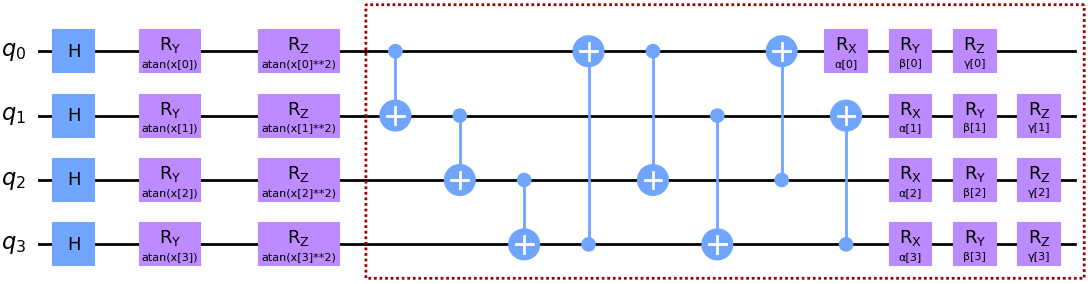
\includegraphics[width=16cm]{lib/graphics/paper_1.png}
    \caption*{Test-\ac{VQC} 1 entnommen aus~\cite{Chen2022}}
    \label{abb:paper1}
\end{figure}

\textbf{Paper 2:}
\begin{figure}[htb]
    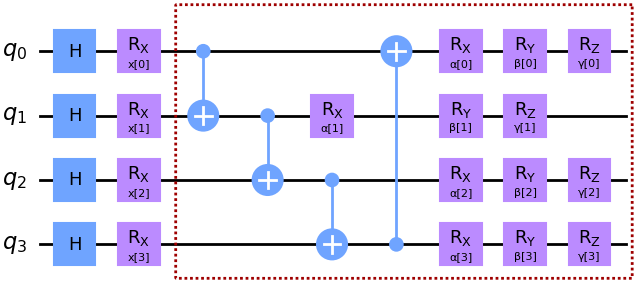
\includegraphics[height=3.9cm]{lib/graphics/paper_2.png}
    \caption*{Test-\ac{VQC} 2 entnommen aus~\cite{Yu2023}}
    \label{abb:paper2}
\end{figure}

\textbf{Paper 3:}
\begin{figure}[htb]
    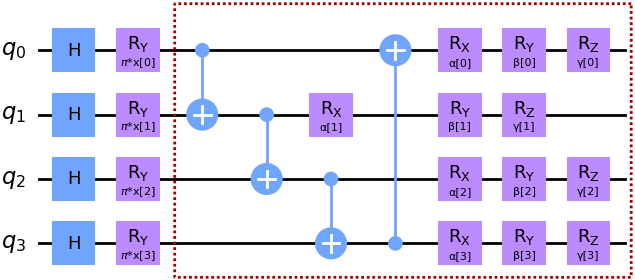
\includegraphics[height=3.9cm]{lib/graphics/paper_3.png}
    \caption*{Test-\ac{VQC} 3 entnommen aus~\cite{Qi2021}}
    \label{abb:paper3}
\end{figure}

\textbf{My\_Own:}
\begin{figure}[htb]
    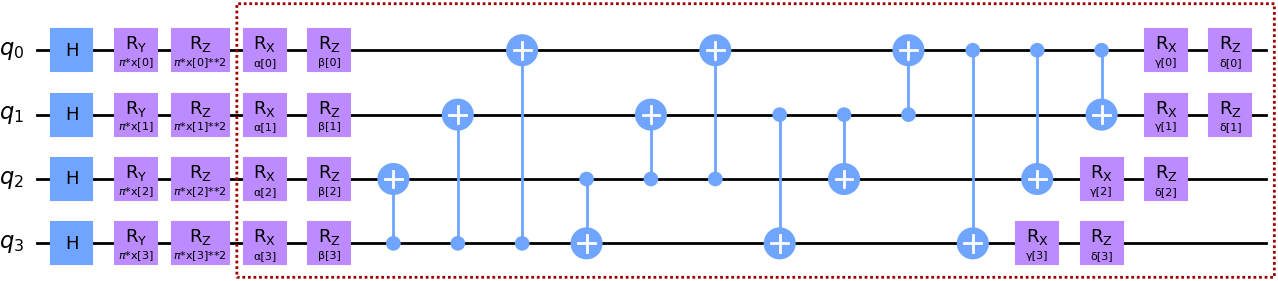
\includegraphics[width=16cm]{lib/graphics/paper_4.png}
    \caption*{Test-\ac{VQC} 4 entnommen aus~\cite{Sim2019} und ~\cite{Chen2022}}
    \label{abb:paper4}
\end{figure}


\anhangteil{Testergebnisse: 4 QLSTM im Vergleich}\label{q_visual}
Lorem Ipsum ist ein einfacher Platzhaltertext für den Druck- und Satzindustrie. Lorem Ipsum hat im Wesentlichen die Norm des Industriestandards seit dem 1500s, als ein unbekannter Drucker eine Hand voll von Typen nahm und sie durcheinander warf, um ein Musterbuch zu machen. Es hat nicht nur fünf Jahrhunderte überlebt, sondern auch den Sprung in die elektronische Schriftbearbeitung, ohne wesentlich zu ändern. Es wurde in den 1960s mit dem Aufkommen von Letraset-Blättern mit Lorem Ipsum-Passagen und mehr kürzlich mit Desktop-Publishing-Software wie Aldus PageMaker einschließlich Versionen von Lorem Ipsum popularisiert.



\newpage\label{q_visual}

\anhang{Entwicklungsumgebung}

\textbf{Hardware und Software}

MacBook 2019;
2,4 GHz 8-Core Intel Core i9,
32 GB RAM

Anaconda Navigator 2.3.2

Visual Studio Code: 1.82.2 (Universal)
\\

\textbf{Python Umgebung}
 
\begin{tabular}{|l|l|}
    \hline
    \textbf{Bibliothek} & \textbf{Version} \\
    \hline
    ipykernel & 6.23.1 \\
    ipython & 8.13.2 \\
    ipywidgets & 8.0.6 \\
    matplotlib & 3.7.1 \\
    matplotlib-inline & 0.1.6 \\
    numpy & 1.23.5 \\
    pandas & 2.0.1 \\
    pip & 23.1.2 \\
    qiskit & 0.43.0 \\
    qiskit-aer & 0.12.0 \\
    qiskit-ibmq-provider & 0.20.2 \\
    qiskit-machine-learning & 0.6.1 \\
    qiskit-terra & 0.24.0 \\
    torch & 2.0.1 \\
    torchmetrics & 0.11.4 \\
    \hline
\end{tabular}
\label{conda}

\clearpage


%%% Quellenverzeichnisse %%%
\literaturverzeichnis
\cleardoublepage

%%% Erklärung %%%
\clearpage

\thispagestyle{empty}

{\LARGE\textsf{\textbf{Erklärung}}\bigskip}

% \typMeinerArbeit und \themaMeinerArbeit werden in src/config.tex definiert
Ich versichere hiermit, dass ich die vorliegende Arbeit mit dem Thema: \emph{\bootstrapPaperTitle} selbstständig verfasst und keine anderen als die angegebenen Quellen und Hilfsmittel
benutzt habe. Ich versichere zudem, dass die eingereichte elektronische Fassung
mit der gedruckten Fassung übereinstimmt.

\vspace{3cm}

\begin{center}
    \begin{tabular}{ccc}
        (Ort, Datum) & \hspace{0.3\linewidth} & (Unterschrift)
    \end{tabular}
\end{center}


\end{document}